\documentclass[dvipdfmx]{jarticle}
\usepackage{graphicx}
\usepackage[top=30truemm,bottom=30truemm,left=25truemm,right=25truemm]{geometry}
\usepackage{listings,jvlisting}
\usepackage{url}

\lstset{
  basicstyle={\ttfamily},
  identifierstyle={\small},
  commentstyle={\smallitshape},
  keywordstyle={\small\bfseries},
  ndkeywordstyle={\small},
  stringstyle={\small\ttfamily},
  frame={tb},
  breaklines=true,
  columns=[l]{fullflexible},
  numbers=left,
  xrightmargin=0zw,
  xleftmargin=3zw,
  numberstyle={\scriptsize},
  stepnumber=1,
  numbersep=1zw,
  lineskip=-0.5ex
}

\begin{document}
\begin{titlepage}
    \begin{center}
        {\huge 情報科学実験B 課題3レポ―ト}
        \vspace{180pt}\\
        \begin{tabular}{rl}
            氏名 & 山久保孝亮\\
            所属 & 大阪大学基礎工学部情報科学科ソフトウェア科学コース\\
            メールアドレス & u327468b@ecs.osaka-u.ac.jp\\
            学籍番号 & 09B22084\\
            提出日 & \today\\
            担当教員 & 松本真佑,小南大智
        \end{tabular}
    \end{center}
\end{titlepage}
\section{システムの仕様}
今回作成した課題3Eではプッシュスイッチを開放した時にきらきら星を演奏する.また,プッシュスイッチを押下するまでは無音である.演奏が終了すると1秒間音を鳴らさず,その後再び演奏を再開するということを繰り返す.
また,すべての音と音の間に休止を挟むようにした.これによって同じ音が連続してしまった際に音の切れ目がわからなくなってしまうことを回避している.
\section{ハードウェア回路}
ハードウェア回路は以下の図1のとおりである.
\begin{figure}[h]
    \centering
    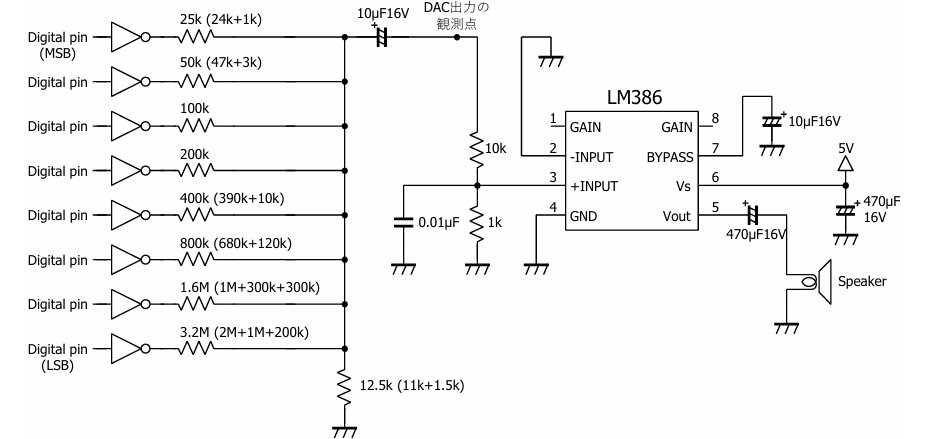
\includegraphics[width=8cm]{kairo.png}
    \caption{D/Aコンバータとアンプの回路図}
\end{figure}
\\上図左部のDigital pinのLSBからMSBまでをArduinoのD2からD9に差し込んだ.
プッシュスイッチに関しては課題1のチャタリング防止回路を利用した.\cite{0}チャタリング防止回路を採用した理由は,プッシュスイッチの開放のタイミングを正確に把握するためである.
\section{制御プログラム}
制御プログラムはsetup関数,loop関数,ISRに大きく分けられる.
\begin{description}
    \item[setup関数]\mbox{}\\
    ここでは初期設定を行った.初期状態では音を鳴らさないようにしなければならないので,TIMSK1のOCIE1Aを0に設定することで割り込みが発生しないようにした.また,OCR1Aが最初に鳴らす音であるscale[0]に設定した.
    scaleは演奏する曲の音階が入力された配列であり,休止の際の値は655
    \item[loop関数]\mbox{}\\
    ここでは音階と音を出力する長さの制御を行った.具体的には以下のフローチャートに従って処理が実行される.
    以下ではスイッチが解放されたときのループの処理とそれ以降のループの処理を記述する.スイッチが解放されると,offbutton関数を最初に実行し,changeというフラグを使用することで非トラッキング処理でスイッチの開放を検出する.offbutton関数は
    グローバル変数として前回のループのボタンの状態を記憶して起き,直前は押していたが現在は押していないときにフラグを1にする関数である.
    また, フラグが立っていれば割り込みを有効にする.これによってスイッチを開放した時に音を鳴るようになる.次にmillis関数を使って現在の時間を取得し初期値が0である変数nowとの差がlength[0]の値以上かどうかを判定する.
    lengthはそれぞれの音の長さを格納する配列である.この条件式が満たされていない間はOCR1Aが初期値のscale[0]に設定されるので  最初に指定している音階の音が鳴り続ける.条件式が満たされた場合,nowの値がその時のmillis関数の値に設定され
    初期値が0のcountの値が1インクリメントされ,OCR1Aが初期値のscale[1]に設定される.それ以降のループでは新たに設定されたnowとmillis関数の値の差がlength[count]以上になるかを判定してOCR1Aをscale[count]に設定し,countをインクリメントしていく作業をcountが84になるまで繰り返す.
    84というのは音階と休止をすべて合わせた数である.単純な音階と最後の休止を実現するのであれば43個で十分であったが,システムの仕様で記述した通り,それぞれの音の間に短い休止をいれることで音の切れ目を表現するために採用した.84になればOCR1Aをscale[0]に設定することで繰り返し楽曲を演奏する機能を実現した.
\end{description}
\section{課題3Aの理想値の計算}
図1のD/Aコンバータとアンプの回路図における左側の8個の抵抗は並列回路であるので、これらの合成抵抗Rの計算式は以下のようになる.
\begin{equation}
\frac{1}{R}=\frac{1}{25k}+\frac{1}{50k}+\frac{1}{100k}+\frac{1}{200k}+\frac{1}{400k}+\frac{1}{800k}+\frac{1}{1.6M}+\frac{1}{3.2M}=\frac{51}{640000}
\end{equation}
即ちRの値は,
\begin{equation}
    R=\frac{640000}{51}
\end{equation}
また,図1の12.5kΩの抵抗は分圧回路と見なせるので\cite{0},のこぎり波の最大電圧であるVoutは,
\begin{equation}
    Vout = \frac{R}{R+12.5k}*5 = 
\end{equation}
\section{工夫点}
今回私が工夫した点としては,曲の演奏情報を配列に格納し,loop関数の構造をシンプルにした点である.この工夫の利点としては,配列の音階や音の長さの情報を変更してもプログラムが動作するので
今回実装したきらきら星以外の曲を演奏しようとする場合配列を変更するだけでよいということである.
\section{考察}
今回の課題を通して私が考察したのは,Arduinoを使って和音を出力することができないかということである.和音について考えた理由は,楽曲を演奏するにあたって和音を使用することで表現の範囲が広がるためである.
最初に私は複数のスピーカとfork()のようなものを使用し複数のスピーカで異なる音階を同期して鳴らすことで和音を実現できるのではないかと考えた.
\section{感想}
今回の課題ではハードウェアの問題なのか,ソフトウェアの問題なのかを見極めることが非常に難しかった.問題を分割して個々の問題の状態を観察することができるのかを考える力は
授業内の課題に限らず,生きていく上でも非常に有用な能力であると感じた.
\section{謝辞}
動作確認や質問対応をしてくださった教授及びTAの皆様,有難うございました.引き続き課題4でも宜しくお願いします.
\begin{thebibliography}{99}
    \bibitem{0} 2024年度情報科学実験B指導書
\end{thebibliography}
\end{document}